\documentclass{article}

\usepackage{fancyhdr} % Required for custom headers
\usepackage{lastpage} % Required to determine the last page for the footer
\usepackage{extramarks} % Required for headers and footers
\usepackage[usenames,dvipsnames]{color} % Required for custom colors
\usepackage{graphicx} % Required to insert images
\usepackage[fleqn]{amsmath}
\usepackage[cs4size,UTF8,winfonts,heading=true]{ctex}
\usepackage{tikz,pgfkeys,pgf,pgfplots}
\usepackage{times}
\usepackage{floatrow}
\usepackage[labelfont=bf,labelsep=quad]{caption}
\setlength{\parindent}{4em}
\addtolength{\parskip}{3pt}
\usepackage[compact]{titlesec}         % you need this package
\titlespacing*{\subsection}{0pt}{0pt}{0pt} % this reduces space between (sub)sections to 0pt, for example

% Margins
\topmargin=-0.45in
\evensidemargin=0in
\oddsidemargin=0in
\textwidth=6.5in
\textheight=9.0in
\headsep=0.25in
\headheight=13pt

\linespread{1.1} % Line spacing

% Set up the header and footer
\pagestyle{fancy}
\lhead{网络安全一班} % Top left header
\chead{\hmwkClass\ \hmwkTitle} % Top center head
\rhead{3019244283 谢远峰 } % Top right header
\renewcommand\headrulewidth{0.4pt} % Size of the header rule
\renewcommand\footrulewidth{0.4pt} % Size of the footer rule
\renewcommand{\normalsize}{\fontsize{12pt}{\baselineskip}\selectfont}
% \renewcommand{\contentsname}{目录} % Use 目录 instead of Content



%--Edit Title, Author and Date here
\newcommand{\hmwkTitle}{编译原理-词法分析} % Assignment title
\newcommand{\hmwkClass}{} % Course/class
\newcommand{\hmwkClassTime}{\today} % Class/lecture time
\newcommand{\hmwkAuthorName}{网安一班\ 3019244283\ 谢远峰 } % Your name
% \titlespacing*{\subsection} {0pt}{9pt}{0pt}
% \floatsetup[table]{capposition=top}%加上这条命令table环境的caption才会置于表格顶端

\title{
\vspace{2in}
\huge{\textbf{\hmwkClass \  \hmwkTitle}}\\
% \Large\vspace{0.1in}\large{\hmwkSupplement}\\
\vspace{2.5in}
}

\author{\textbf{\hmwkAuthorName}}
\date{\hmwkClassTime}

%----------------------------------------------------------------------------------------

\begin{document}

\maketitle
% \thispagestyle{empty}

% \newpage
% \tableofcontents
\newpage
\subsection*{a}
\noindent
(1)\qquad$A|A \rightarrow \{A\} \leftarrow A$ \\
(2)\qquad$A^* \rightarrow \{\varepsilon , A,AA,\cdots,\text{任意个A的串}\} \leftarrow A^*$ \\
(3)\qquad$A^* \rightarrow \{\varepsilon , A,AA,\cdots,\text{任意个A的串}\} \leftarrow \varepsilon|AA^*$ \\
(4)\qquad$(AB)^*A \rightarrow \{\text{一个A数量比B多1的串}\} \leftarrow A(BA)^*$ \\
\subsection*{b}
\noindent
(1)\text{以01结尾的二进制数}\qquad$(0|1)^*01$\\
(2)\text{能被5整除的十进制数}\qquad$(+|-|\varepsilon)(0|1|2|3|4|5|6|7|8|9)^*(0|5)$\\
(3)\text{包含奇数个0或奇数个1的二进制数}\qquad$1^*0(1^* | 01^*0)^*\text{(奇数个0)}  |\  0^*1(0^* | 10^*1)^*\text{(奇数个1)} $\\
(4)\text{26个英文字母(小写)组成符号串,串中的字母依照字典顺序排列}\qquad$(a|\varepsilon)^*(b|\varepsilon)^*(c|\varepsilon)^*\cdots (z|\varepsilon)^*$\\
\subsection*{c}
\begin{center}
    DFA为$M=\{\{A,B,C,D,E,F\},\{a,b\},\delta ,A,F\}$
\end{center}
\setlength{\abovecaptionskip}{0.cm}
\begin{table}[htb]
    \floatsetup{floatrowsep=qquad,captionskip=3pt} \tabcolsep=14pt
    \begin{floatrow}
        \ttabbox{\caption{NFA确定化}}{%
            \begin{tabular}{|c|c|c|}\hline
                ~                            & $I_a$       & $I_b$       \\\hline
                \{0,1,2,4,7\}$\rightarrow$ A & \{3,6,7,8\} & \{5,6,7,8\} \\\hline
                \{3,6,7,8\}$\rightarrow$ B   & \{8\}       & \{9\}       \\\hline
                \{5,6,7\}$\rightarrow$ C     & \{8\}       & $\phi$      \\\hline
                \{8\}$\rightarrow$ D         & $\phi$      & \{9\}       \\\hline
                \{9\}$\rightarrow$ E         & $\phi$      & \{10\}      \\\hline
                \{10\}$\rightarrow$ F        & $\phi$      & $\phi$      \\\hline
            \end{tabular}}
        \ttabbox{\caption{状态转换矩阵}}{%
            \begin{tabular}{|c|c|c|}\hline
                ~ & a      & b      \\\hline
                A & B      & C      \\\hline
                B & D      & E      \\\hline
                C & D      & $\phi$ \\\hline
                D & $\phi$ & E      \\\hline
                E & $\phi$ & F      \\\hline
                F & $\phi$ & $\phi$ \\\hline
            \end{tabular}}
    \end{floatrow}
\end{table}
\begin{figure}[h]
    \centering
    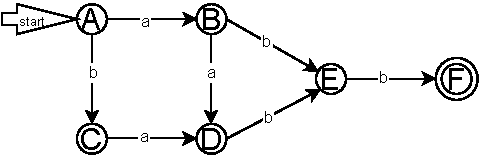
\includegraphics[width=13cm,height=4cm]{1.pdf}
    \caption{状态转换图}
\end{figure}
\clearpage
\subsection*{d}
\begin{flalign*}
    \begin{split}
        &1.\pi_{0}=\{\{S_0,S_1,S_2,S_3\},\{S_4\}\}               \\
        &mov(\{S_0,S_1,S_2,S_3\},a)=\{S_1\}         \\
        &mov(\{S_0,S_1,S_2,S_3\},b)=\{S_2,S_3,S_4\} \\
        &\text{其中$S_0,S_2$接受b到达状态$S_2,S_1$到达状态$S_3,S_3$到达状态$S_4$,所以$S_3$单独一类}\\
        &2.\pi_{1}=\{\{S_0,S_1,S_2\},\{S_3\},\{S_4\}\}               \\
        &mov(\{S_0,S_1,S_2\},b)=\{S_2,S_3\} \\
        &\text{其中$S_0,S_2$接受b到达状态$S_2,S_1$到达状态$S_3$,所以$S_1$单独一类}\\
        &3.\pi_{2}=\{\{S_0,S_2\},\{S_1\},\{S_3\},\{S_4\}\}               \\
        &\text{由以上分析$S_0,S_2$同属一类,合并为一个状态}\\
        &   M=\{\{S_0,S_1,S_3,S_4\},\{a,b\},f,S_0,S_4\}\}
    \end{split}
\end{flalign*}
\ttabbox{\caption{状态转换矩阵}}{%
    \tabcolsep=14pt
    \begin{tabular}{|c|c|c|}\hline
        ~     & a     & b     \\\hline
        $S_0$ & $S_1$ & $S_0$ \\\hline
        $S_1$ & $S_1$ & $S_3$ \\\hline
        $S_3$ & $S_1$ & $S_4$ \\\hline
        $S_4$ & $S_1$ & $S_0$ \\\hline
    \end{tabular}}
\begin{figure}[h]
    \centering
    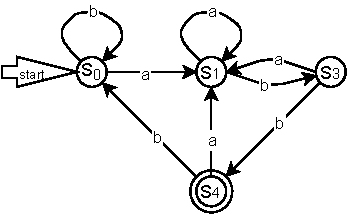
\includegraphics[width=8cm,height=4cm]{2.pdf}
    \caption{DFA最小化图}
\end{figure}
\subsection*{e}
\begin{minipage}[h]{0.7\linewidth}
    \begin{flushleft}
        令狼$\rightarrow W$,羊$\rightarrow S$,白菜$\rightarrow C$,人$\rightarrow P$ \\
        关系集合$\delta$包含关系G(x)人带某物过河,R(x)人带某物返回\\
        状态矩阵表示未过河物体的集合\\
        \begin{align}
            0(PWSC)\rightarrow G(S)\rightarrow 5(WC)   \\
            5(WC)\rightarrow R(\phi)\rightarrow 2(PWC) \\
            2(PWC)\rightarrow G(W)\rightarrow 8(C)     \\
            8(C)\rightarrow R(S)\rightarrow 3(PSC)     \\
            3(PSC)\rightarrow G(C)\rightarrow 7(S)     \\
            7(S)\rightarrow R(\phi)\rightarrow 4(PS)   \\
            4(PS)\rightarrow G(S)\rightarrow 9(\phi)
        \end{align}
    \end{flushleft}
\end{minipage}
\hfill
\begin{minipage}[h]{0.3\linewidth}
    \begin{flushright}
        \ttabbox{\caption{状态矩阵}}{
            \begin{tabular}{|c|c|}\hline
                0    & 1       \\\hline
                PWSC & PWS     \\\hline
                2    & 3       \\\hline
                PWC  & PSC     \\\hline
                4    & 5       \\\hline
                PS   & WC      \\\hline
                6    & 7       \\\hline
                W    & S       \\\hline
                8    & 9       \\\hline
                C    & $\phi $ \\\hline
            \end{tabular}}
    \end{flushright}
\end{minipage}
$$M=\{\{0,1,2,3,4,5,6,7,8,9\},\{S,W,C\},\{G,R\},0,9\}$$
\begin{figure}[ht]
    \centering
    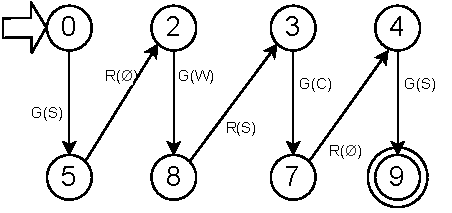
\includegraphics[width=10cm,height=4cm]{3.pdf}
    \caption{状态转换图}
\end{figure}
\end{document}